\chapter{adolecencia y universidad}
\section{universidad}
bueno pues finalmete llege ala universidad en la cual se podria decier que despues de pensar toda mi vida que la escuela era algo facil,
varios profesores de mi universidad
me isieron sentar cabesa porque yo apartir de la secundaria nunca avia reprobado una materia
pero en la universidad en 3 semestres reprobe 6 materias de las cuales solo e podido pasar 4 
y pues creo que aqui fue donde verdaderamente me entro lo que todos me decian, 
la Melalcolia
\begin{figure}[H]
\centering
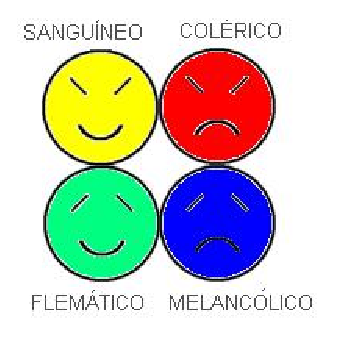
\includegraphics{sixChapter/mela.eps}
\caption{la universidad :(}
\label{universidad}
\end{figure}
pero despues de todo me plante que lo unico que tenia que hacer para sobrebibir en la escuela es lo siguiente:
\begin{enumerate}[1.]
\item entrar a clases
	\begin{enumerate}[a-]
		\item poner atencion
		\item no distraerse 
	\end{enumerate}
\item estudiar 
	\begin{enumerate}[a-]
                \item 30 minutos cada materia
        \end{enumerate}
\item ir a acesorias
\item entre otras
\end{enumerate}
